\documentclass[11pt]{article}
\usepackage{verbatim}
\usepackage{graphicx}

\title{\textbf{COMS 6100 - Homework 11}}
\date{October 18, 2017}
\author{Thomas Goff\\ Middle Tennessee State University}


\begin{document}
\maketitle
\section{Python Implementation}
\verbatiminput{montecarlo.py}
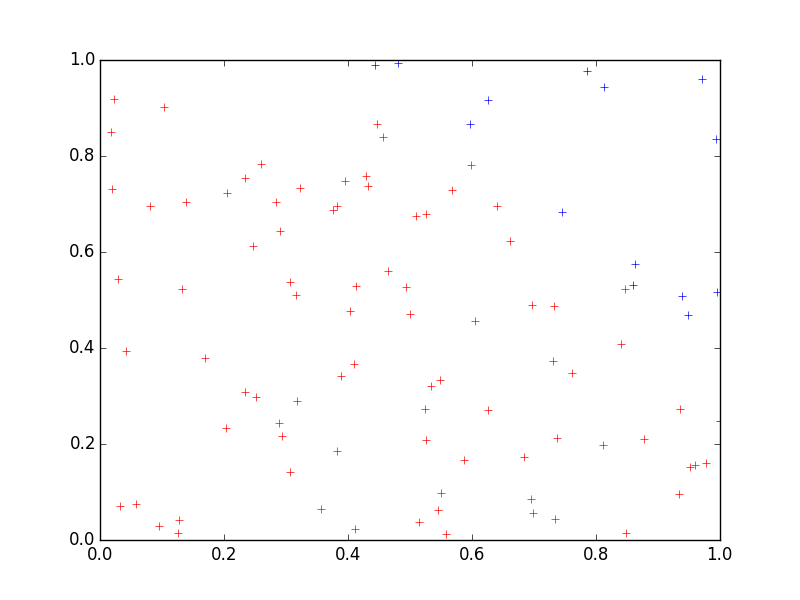
\includegraphics{plot100.png}
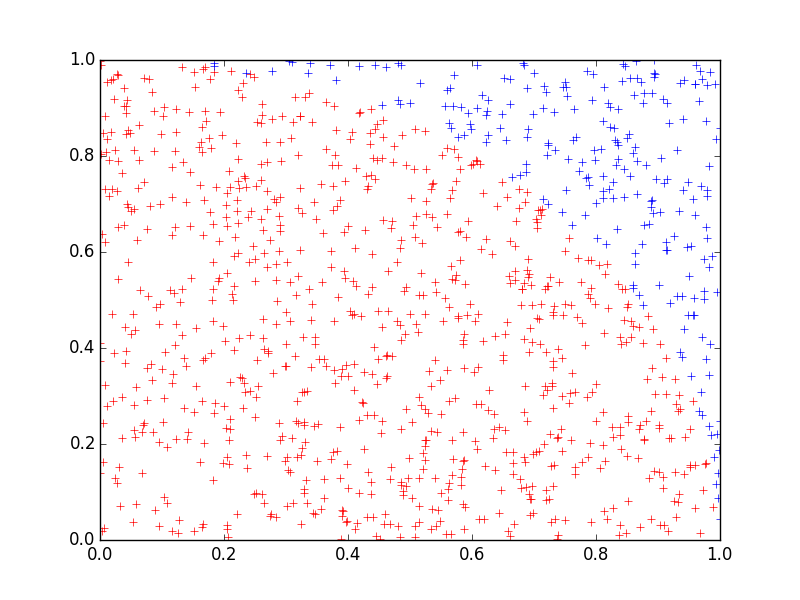
\includegraphics{plot1000.png}
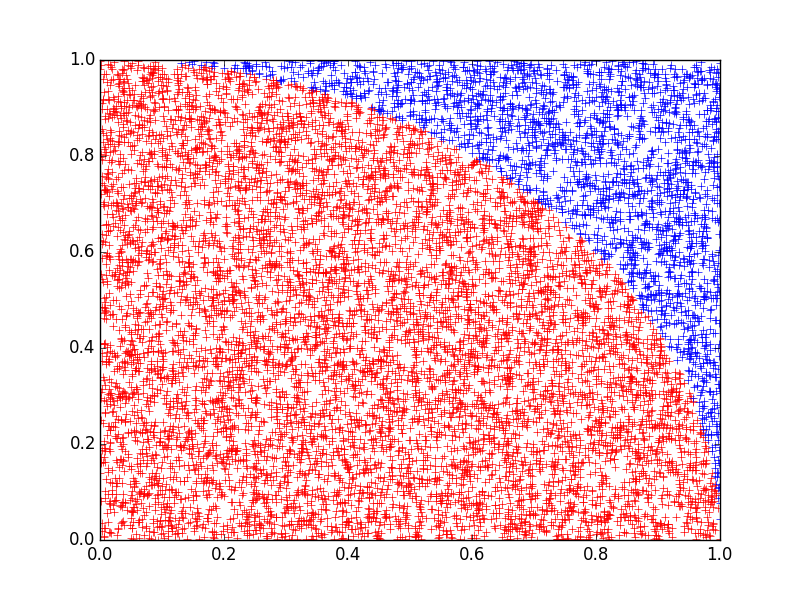
\includegraphics{plot10000.png}
\section{C++ Implementation}
\verbatiminput{mc.cpp}
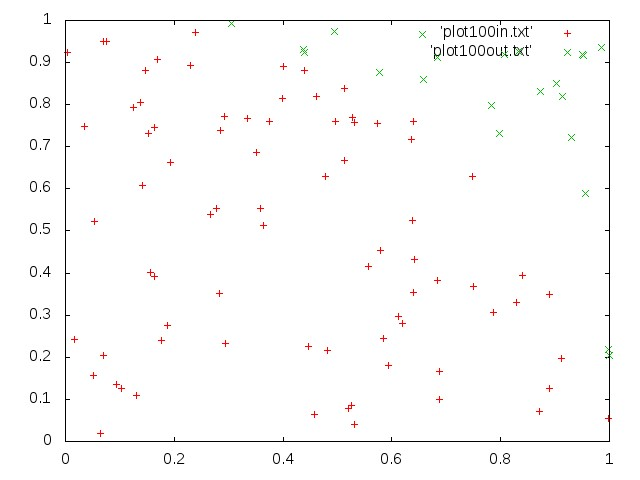
\includegraphics{plot100.jpg}
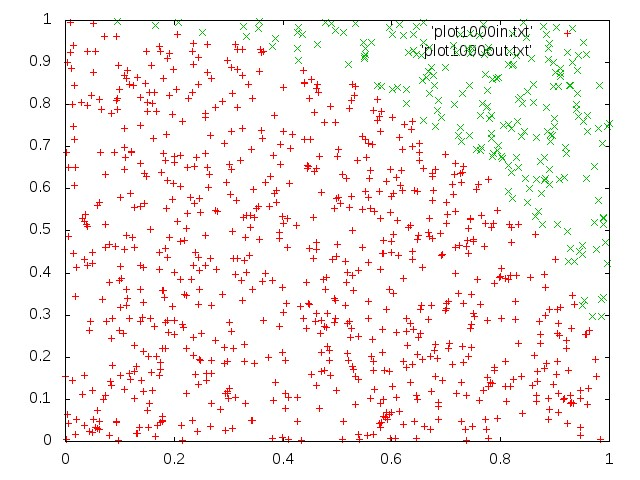
\includegraphics{plot1000.jpg}
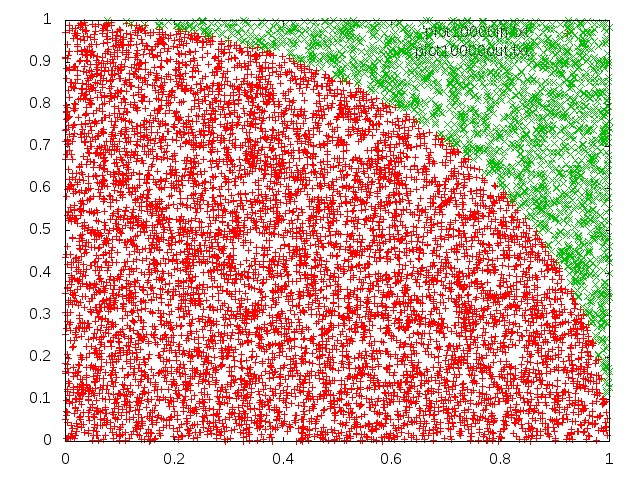
\includegraphics{plot10000.jpg}

\section{Writeup}
This task was very fun and interesting for me.  Implementing the python code was very simple, and didn't require that many lines of code, whereas, including blank spaces and comments, the c++ implementation took almost twice as many lines.  The main issues I ran into at first was not typecasting in python whenever I should have. The biggest issue that I had while implementing the c++ version of the assignment was making sure that all of the std functions that I wanted to use would be included. In order for my c++ code to compile, the -std=c++11 option must be given to g++, because of a certain function that I used while typecasting. Overall, the task was fun in both languages, however, the python implemenation was much quicker to code. On the efficiency side though, the c++ implemenation should be able to execute much more quickly and even use larger values of n.











\end{document}
